\section{Introduction}
Work presented in previous chapters highlighted the much improved \textit{ab initio} decoy quality achievable by restraining the conformational search space with residue-residue contact information. Furthermore, the data also highlighted that this improvement extends AMPLE's tractability of achieving structure solution for more challenging targets. However, the data also indicated that AMPLE's current protocol is not tailored towards decoy sets with overall much higher accuracy. Decoy sets with correctly predicted folds (average \gls{tmscore} $>0.5$ per 1,000 decoys) did not generate any or many ensemble search models leading to \gls{mr} structure solution. It also became apparent that certain decoy sets contained few high-quality decoys that were lost in the process of clustering, since non of the top-10 SPICKER clusters contained that fold.

Beyond the limitations observed in AMPLE, \textit{ab initio} decoy similarity in exceptional cases approaches a near-identical fold (RMSD $<1.5$\AA) to the crystallised one. Although challenging by current means to identify these decoys, it is of great interest since these decoys might be sufficient by themselves as \gls{mr} search models. Contact information, which was used to restrain the folding protocol, might provide enough information to drive such filtering. Indeed, \textcite{De_Oliveira2017-gj} found that long-range residue-residue contact pair satisfaction correlates well with decoy quality. Additionally, \textcite{Adhikari2018-lj} use long-range contact satisfaction routinely in CONFOLD2 to exclude the worst decoys amongst the set predicted ones.

Thus, this chapter focuses on exploring alternative strategies of decoy selection in AMPLE, and if contact information can be used beyond the distance-restraint application in \textit{ab initio} protein structure prediction.

\section{Materials \& Methods}
\subsection{Target selection}
The dataset for this study consisted of 113 ROSETTA decoy sets generated throughout the works outlined in previous chapters. The 113 decoy sets covered all targets in the ORIGINAL (\cref{table:appendix_dataset_original}), PREDICTORS (\cref{table:appendix_dataset_predictors}) and TRANSMEMBRANE (\cref{table:appendix_dataset_transmembrane}) datasets. Top-$L$ ($>5$ residues sequence separation) CCMPRED \cite{Seemayer2014-zp}, PCONSC2 \cite{Skwark2014-qp}, METAPSICOV STAGE 1 \cite{Jones2015-vq} and MEMBRAIN \cite{Yang2013-bf} contact pairs were used in combination with the \textit{FADE} energy function to restrain the \textit{ab initio} structure prediction process.

\subsection{Computation of range-specific satisfaction scores}
The satisfaction of short- ($>6$ residues sequence separation), medium- ($>12$ residues sequence separation) and long-range contact pairs ($>23$ residues sequence separation; see \cref{sec:methods_longrange_satisfaction}) were computed for each decoy in each set. Hereby, the contact pairs of the original set of contact pairs used to restrain the \textit{ab initio} structure prediction protocol were extracted, matched against the contact pairs extracted from individual decoys and the contact pair range-specific satisfaction score evaluated. 

\subsection{Decoy subselection}
Each set of decoys was then ranked in descending order by their long-range contact pair satisfaction scores and the $n$ decoys with the lowest scores removed from each set. The number of decoys to remove $n$ were selected using a number of different strategies:

\begin{itemize}
    \item \textit{NONE}: leave the original set unchanged
    \item \textit{LINEAR}: remove the worst 500 decoys
    \item \textit{CUTOFF}: remove all decoys with a score of $<0.287$ 
    \item \textit{SCALED}: remove all decoys with a scaled score of $<0.5$, where the scaled score is score divided by set average
\end{itemize}

The fixed definition in the \textit{CUTOFF} strategy was determined by \textcite{De_Oliveira2017-gj}. The scaled score used by the \textit{SCALED} strategy was computed by dividing each decoy's long-range contact pair satisfaction by the set's average.

\subsection{Molecular Replacement}
To evaluate the benefits of such subselection to \gls{mr} in AMPLE, a subset of 35 decoy sets (spanning 35 unique targets) were processed as described above and subjected to AMPLE v1.2.0 and CCP4 v7.0.28. Default options were chosen with few exceptions: decoys in all 10 clusters were used, subcluster radii thresholds were set to 1 and 3\AA, and side-chain treatments were set to \texttt{polyala} only. This change in protocol was shown to be advantageous in most cases by Jens Thomas (PhD Thesis), and thus trialled in this context. 

To allow comparability of these results to previous AMPLE runs, an additional condition was added, namely \textit{NONE\_classic}. The decoy set from the \textit{NONE} strategy was hereby subjected to the AMPLE protocol with default settings.

Each \gls{mr} run was assessed using the criteria defined in \cref{sec:methods_mr_success}.

\section{Results}
This chapter focuses on identifying further uses of predicted residue-residue contact pairs in unconventional \gls{mr}. In particular, the exclusion of \textit{ab initio} decoys by their contact satisfaction scores is under investigation. A total of 113 decoy datasets were used to identify potential means of identifying the best or worst decoys. Furthermore, three strategies were trialled alongside two standards to test the viability of excluding the worst decoys in ensemble search model preparation in AMPLE.

\subsection{Satisfaction of long-range contact pairs evaluates decoy quality}
\textcite{Kosciolek2014-bt} previously identified a correlation between the TM-score of a decoy and its fraction of satisfied contact pairs. Albeit the striking positive correlations (short-range:$\rho=0.50$; medium-range:$\rho=0.57$; long-range:$\rho=0.87$) for top-1 decoys, the study by \textcite{Kosciolek2014-bt} was limited to 10 representative targets with a maximum chain length of 158 residues. Furthermore, FRAGFOLD \cite{Jones2001-mc} was used for \textit{ab initio} protein structure prediction, a method with inferior performance to ROSETTA \cite{Rohl2004-dj} when using the decoys in unconventional \gls{mr} (see \cref{chap:alternate_abinitio_protocols}). Thus, the more diverse set of decoys generated in this study might be more representative in determining a correlation between decoy TM-scores and contact pair satisfaction.

A correlation analysis with 35 ROSETTA decoy sets representing 35 globular and transmembrane targets shows a positive linear correlations between a decoy's TM-score and short-, medium- and long-range contact satisfaction (\cref{table:ample_decoys_tmscore_consat}). Furthermore, separating the correlation analysis of all targets by fold classification reveals that all-\textalpha, mixed \textalpha-\textbeta\ and transmembrane protein targets show the strongest positive correlations for long-range contact satisfaction (\cref{table:ample_decoys_tmscore_consat}). All-\textbeta\ and mixed \textalpha-\textbeta\ decoy sets show the strongest correlations for short- and medium-range contact satisfaction, whereby the former shows a stronger positive correlation between the decoy's TM-score and its medium-range contact satisfaction than its long-range contact satisfaction (medium-range:$\rho=0.54$; long-range:$\rho=0.50$) (\cref{table:ample_decoys_tmscore_consat}). Notably, the decoys of transmembrane protein targets show no correlation between TM-score and short-range contact satisfaction ($\rho=0.08$; \cref{table:ample_decoys_tmscore_consat}).

\begin{table}[H]
  \centering
  \caption[Correlation analysis between decoy TM-score and contact satisfaction]{Pearson's \gls{cc} analysis between a ROSETTA decoy's TM-score and short-, medium- and long-range contact satisfaction. Probability values for all \textrho coefficients is $<0.01$.}
  \label{table:ample_decoys_tmscore_consat}
  \begin{tabularx}{\textwidth}{X X X X}
      \hline
      \multirow{2}{*}{\textbf{Target class}} & \multicolumn{3}{c}{\textbf{Pearson's \gls{cc}}} \\ \cline{2-4}
      & Short-range   & Medium-range  & Long-range \\
      \hline
      all                               & 0.11          & 0.18          & 0.64 \\
      all-\textalpha                    & 0.30          & 0.44          & 0.69 \\
      all-\textbeta                     & 0.40          & 0.54          & 0.50 \\
      mixed \textalpha-\textbeta        & 0.42          & 0.55          & 0.69 \\
      transmembrane                     & 0.08          & 0.48          & 0.70 \\
      \hline
  \end{tabularx}
\end{table}

Following on from the correlation analysis, a linear regression model was fitted to individual subsets of the data used for the correlation analysis to see if a decoy's TM-score could be predicted from its contact satisfaction score. However, weak coefficients of determination indicate that only some cases show models with reasonably good fits to the data (\cref{fig:ample_decoys_smlrcstmfold}). Nevertheless, all models further support the positive linear correlations between a decoy's TM-score and its range-dependent contact satisfaction. Interestingly, the strongest and best fits of the linear regression model to its corresponding data is for long-range contact pairs, where the linear regression models are also near identical between the different fold categories (\cref{fig:ample_decoys_smlrcstmfold}).

\begin{figure}[H]
	\centering
	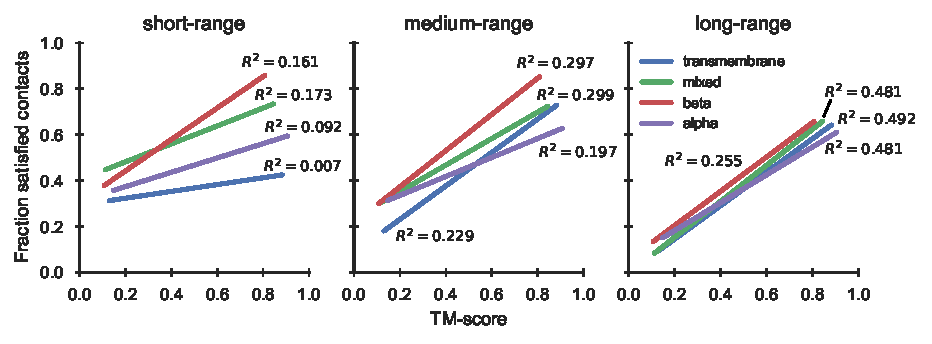
\includegraphics[width=\textwidth]{ample_decoys_smlrcstmfold.pdf}
        \caption[Linear regression model between decoy TM-score and contact satisfaction]{Linear regression model fitted to decoy TM-scores and corresponding fractions of satisfied, range-dependent contacts. Targets were further separated by fold classification. Ceofficients of determination ($R^2$-values) added alongside each regression model.}
	\label{fig:ample_decoys_smlrcstmfold}
\end{figure}

An analysis of the correlation between the TM-score and long-range contact satisfaction of individual decoy sets further highlights the potential to subselect decoy sets by their long-range contact satisfaction. Thirty decoy sets show statistically significant positive correlations between decoy TM-scores and their long-range contact satisfaction ($\rho$-values in range of 0.09 to 0.97 with p-value $<0.01$). A singleton ROSETTA decoy set, derived for the Glycolipid transfer protein with \gls{pdb} ID 2eum and restrained with METAPSICOV STAGE 1 contact data, shows a weak negative correlation ($\rho=-0.10$, $p<0.01$). The remaining four decoy sets, derived for targets with \gls{pdb} IDs 1chd, 1gm4, 2x6u and 3ouf and restrained with METAPSICOV STAGE 1 contact data except for 2x6u (PCONSC2), show no statistically significant correlation between the TM-score and long-range contact satisfaction of the decoy sets. 

A further subdivide of the previously presented data by metapredictor highlights that no predictor outperforms the others. Decoy sets from all metapredictors result in decoy sets with stronger and weaker correlations. Similarly, target chain length and fold do not show overall stronger or weaker correlations. 

So far, all analyses focused on entire sets of decoys (1,000 decoys per set); however, it is often desirable to know if we could better estimate the accuracy of the best decoy by some measure. \textcite{Kosciolek2014-bt} demonstrated strong positive correlations for short-, medium- and long-range contact satisfaction with a decoy's corresponding TM-score. In this work, these findings are confirmed albeit the strength of the correlation for long-range contact satisfaction is much weaker than observed previously (short-range: no correlation; medium-range:$\rho=0.52$; long-range:$\rho=0.69$) (\cref{fig:ample_decoys_smlrcstmtop1}). The weak positive correlation for short-range contact satisfaction is statistically non-significant, and thus cannot be validated. 

\begin{figure}[H]
	\centering
        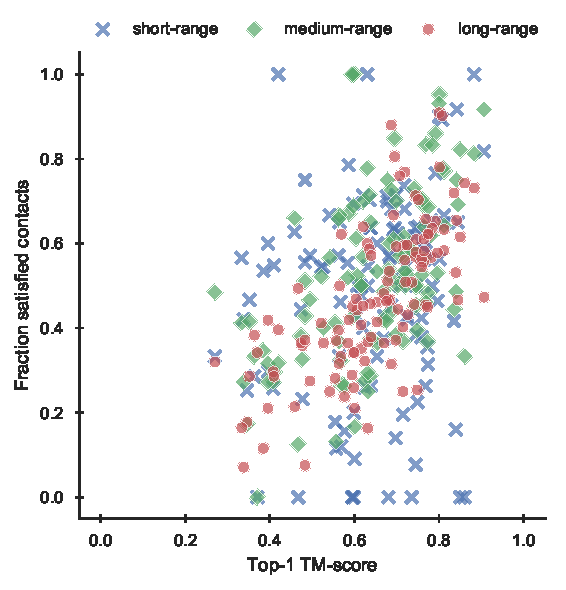
\includegraphics[width=0.7\textwidth]{ample_decoys_smlrcstmtop1.pdf}
        \caption[Top-1 decoy TM-score and contact satisfaction analysis]{Analysis of the relationship between TM-score and contact satisfaction for the top-1 decoy (as ranked by TM-score) in each decoy set.}
	\label{fig:ample_decoys_smlrcstmtop1}
\end{figure}


% - How many decoys do we exclude for the different selection criteria?
% - How does the correlation affect the selection of decoys?
% - How do the exclusion conditions affect the quality measures of our decoy sets?
% - How does the selection impact AMPLE ensemble search model generation?
% - How does decoy exclusion impact MR?
